\subsection{The Measurement Library}
\label{ss:dataflow}

NetMap uses a dedicated server for collecting and storing the performance
measurements (see figure \ref{fig:servers}), so game developers do not need to
worry about securely storing and forwarding the sensitive data, and do not need
to provision for the bandwidth required by the data uploads.

\begin{figure}[hbtp]
  \center{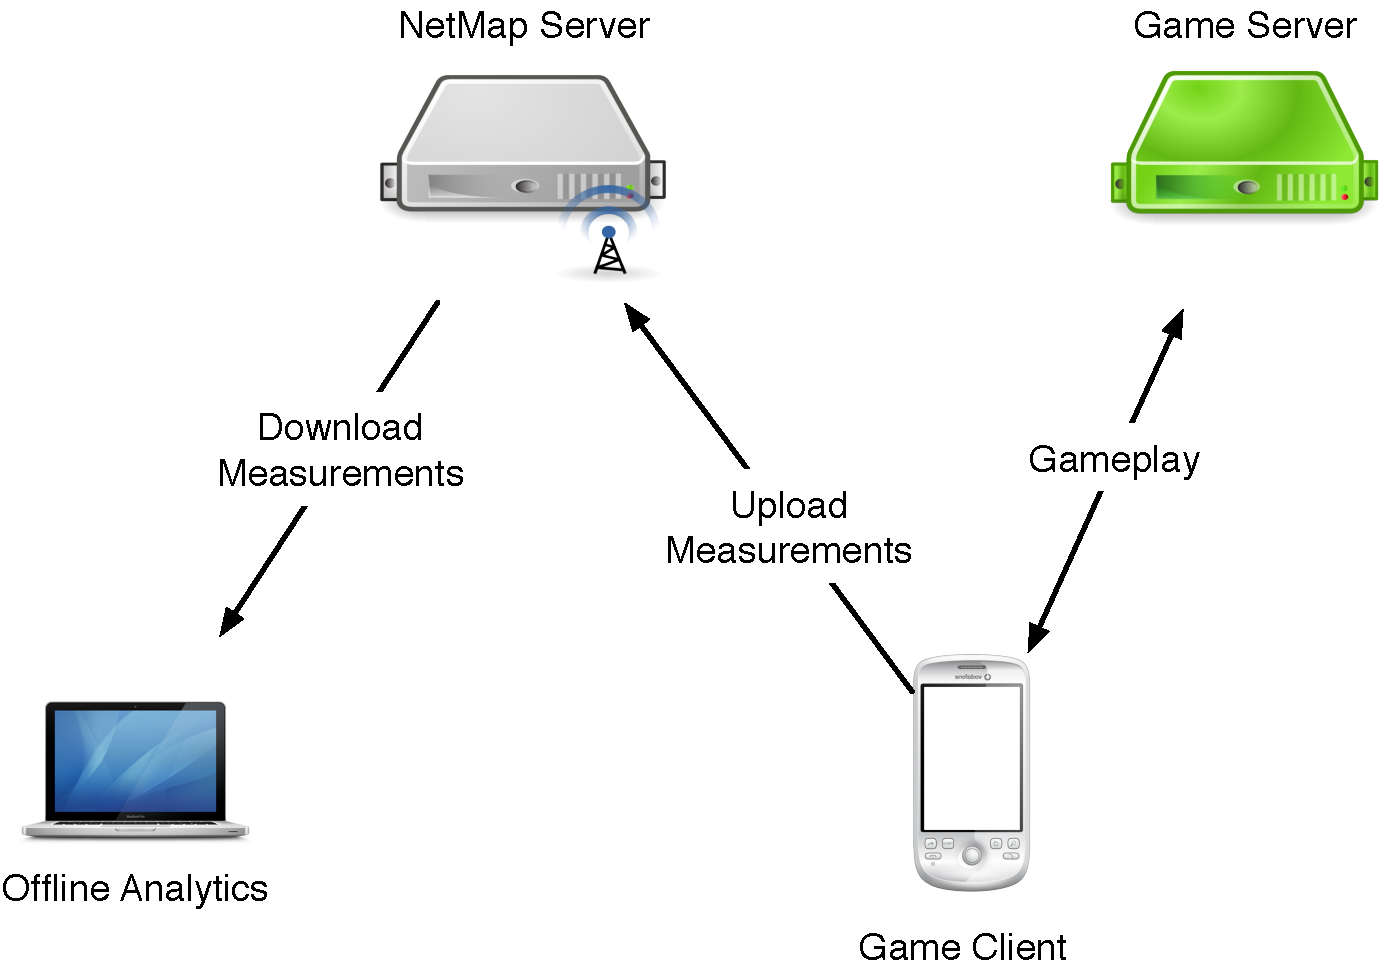
\includegraphics[width=85mm]{figures/servers.pdf}}
  \caption{
    The NetMap platform has a dedicated server for storing network
    performance measurements, and the data is analyzed offline.
  }
  \label{fig:servers}
\end{figure}

The NetMap platform includes an Android library that manages the
straight-forward (but tedious) aspects of measuring network performance and
uploading the data to the NetMap server. We envision that when a player takes
an action in a game, the game code will call our library and ask it to collect
a performance measurement. Powerful moves (such as firing a very powerful
weapon) would trigger the collection of more battery-intensive measurements.
The measurement data is not uploaded to the NetMap
right away, so that the game can use all the player's (potentially limited)
wireless Internet bandwidth, so that the data upload is not charged against
the player's cellular Internet data quotas, and so that we do not burden the
player's mobile device battery. Instead, we queue up the data in a SQLite
database on the player's device, and we wait until the device is connected to a
WiFi network and its charger is plugged in. Under the right circumstances, all
the data queued up in SQLite is uploaded to the measurement server.


\begin{figure}[hbtp]
  \center{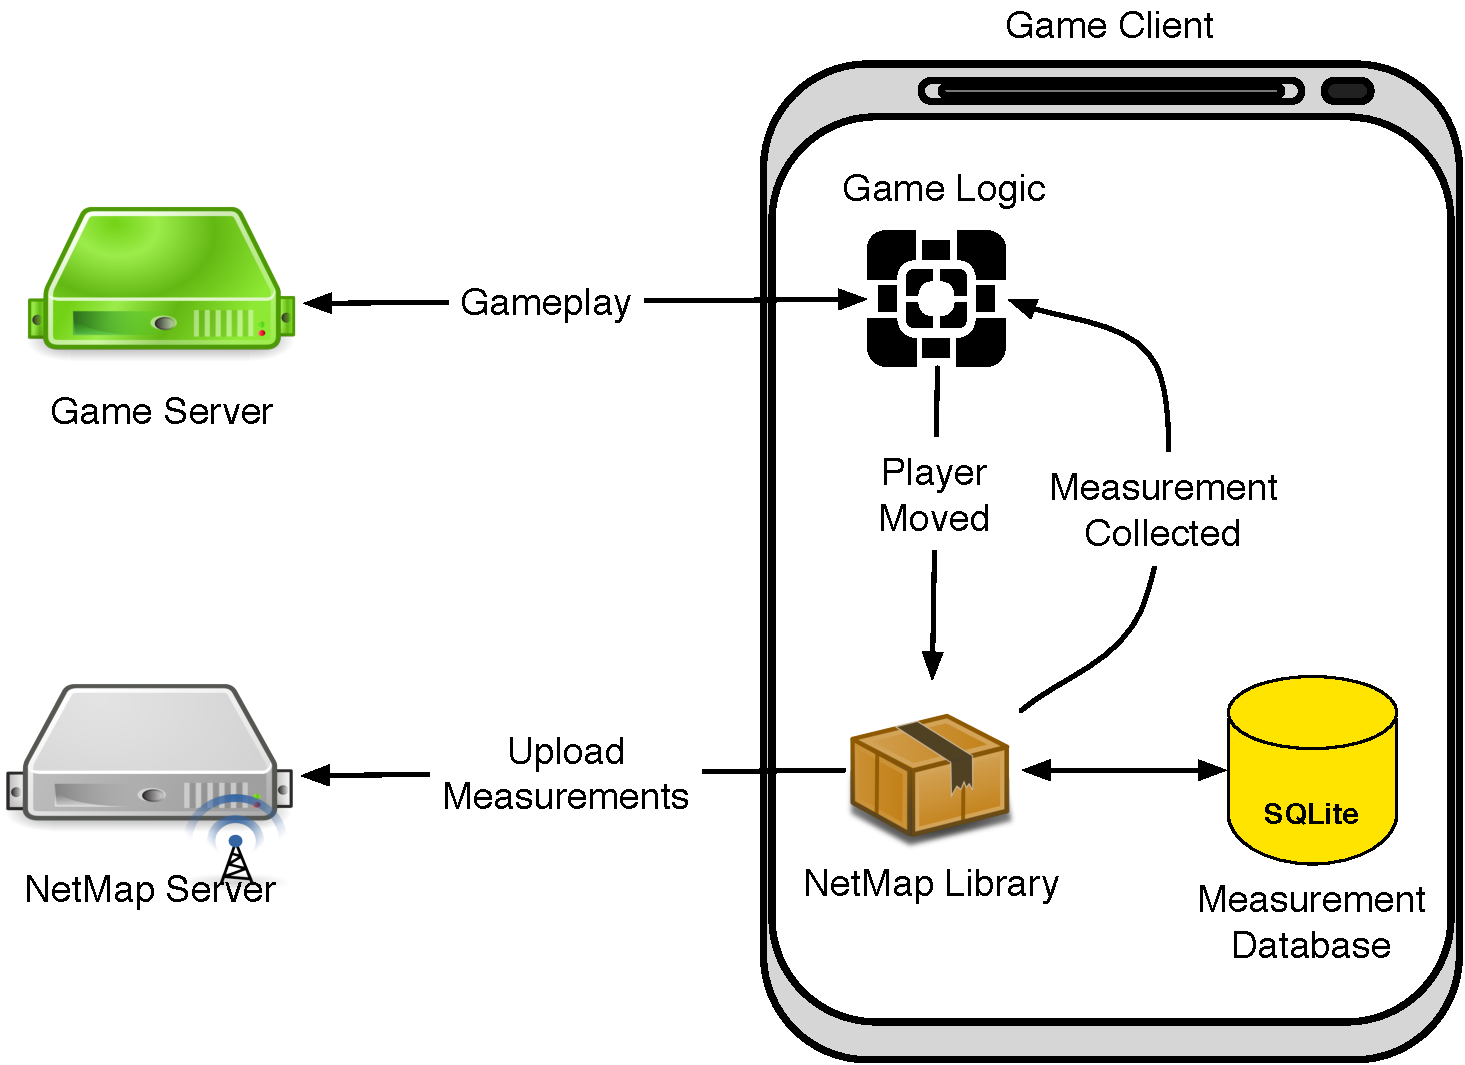
\includegraphics[width=85mm]{figures/dataflow.pdf}}
  \caption{
    The flow of measurement data inside a game client
  }
  \label{fig:dataflow}
\end{figure}

Table \ref{table:api} shows the API exposed by the NetMap measurements library
to the game client code. The \texttt{measure} and \texttt{upload} methods
perform the operations described above, while \texttt{powerSource} and
\texttt{networkSource} help the game client decide when to upload the queued
measurement data to the NetMap server. We expect that most game clients will
upload data when the phone is using a charger and a WiFi network.

\begin{table}[hbtp]
\begin{tabular}{|p{6.25cm}|p{1.5cm}|}
\hline
\textbf{class NetMap}\\
\hline
\hline
measure(\textbf{String} \textit{what}) : String \textit{digest}\\
\hline
upload() : \textbf{boolean} \textit{hasMoreData}\\
\hline
\hline
powerSource() : \textbf{PowerSource}\\
\hline
networkSource() : \textbf{NetworkSource}\\
\hline
location() : \textbf{Location}\\
\hline
\hline
initialize(\textbf{Context} \textit{androidContext})\\
\hline
configure(\textbf{String} \textit{userToken})\\
\hline
trackLocation(\textbf{Boolean} \textit{enabled})\\
\hline
\end{tabular}
\caption{
  The NetMap measurement library API
}
\label{table:api}
\end{table}

The performance measurements are tied to the user's location, so we ask game
clients to call \texttt{trackLocation(\textbf{true})} before performing network
measurements. In return, game code can call \texttt{location} to obtain the
user's location, and game developers do not need to implement their own
location tracking code. We expect that most game clients will call
\texttt{trackLocation(\textbf{true})} when their UI becomes the foreground
activity, and will call \texttt{trackLocation(\textbf{false})} when the game UI
loses the player's focus. This approach supplies location-based games with the
information they need for their UI, and ensures that measurements will have
fresh location information. To be on the safe side, the NetMap analytics code
discards measurements whose location timestamp is significantly older than the
measurement timestamp.

The API also includes asynchronous variants of \texttt{measure} and
\texttt{upload}, an evented interface for changes to \texttt{powerSource},
\texttt{networkSource} and \texttt{location}, as well as JSON-producing
variants of the last 3 functions, for easy integration with JavaScript.

\subsection{The NetMap Server}

The network performance measurement data collected by the NetMap library is
uploaded to the NetMap server, which stores the data for future analysis. We
hope and expect that all the games using the NetMap platform will upload their
measurements to our server. However, our library has an option of changing the
upload server URL, to facilitate game development.

The NetMap server tracks the game that uploaded each piece of measurement data,
and can provide a leaderboard that shows which games have contributed the most
to the network map. Game developers register the information in Table
\ref{table:metrics-app} with the NetMap server and receive an application ID
and secret HMAC key, which they use according to Figure \ref{fig:user-token}
to issue tokens for their players. A user token uniquely identifies the game
and the user that created the measurement, and a game cannot issue tokens on
behalf of another game without knowing its secret key. This allows the NetMap
server to discard a player's data, if the player is found cheating. Our
platform can also discard an entire game's data, if there are signs that the
game code is misbehaving.

\begin{table}[hbtp]
\begin{tabular}{|p{2.00cm}|p{5.50cm}|}
\hline
\textbf{Name} & user-friendly name for leaderboards \\
\hline
\textbf{Backend} & HTTP URL that receives callbacks \\
\hline
\textbf{Email} & developer contact information \\
\hline
\hline
\textbf{App ID} & unique identifier for an application \\
\hline
\textbf{App Secret} & HMAC key \\
\hline
\end{tabular}
\caption{
  Per-application data maintained by the NetMap server. A game developer
  registers her game's name, backend URL and e-mail with the NetMap server, and
  receives an application ID and secret.
}
\label{table:metrics-app}
\end{table}

In the user token generation process illustrated by Figure
\ref{fig:user-token}, each game is responsible for managing its own space of
user IDs, and the NetMap servers treat user IDs as opaque alphanumeric strings.
Our process has the advantage that game servers can issue user tokens that the
NetMap servers can validate, without the need for any synchronization. The main
disadvantage of this design is that user IDs are exposed to game clients, so
we expect that security-conscious game clients will either generate
pseudo-random user IDs, or will encrypt the user IDs exposed to the NetMap API.

\begin{figure}[hbtp]
  \center{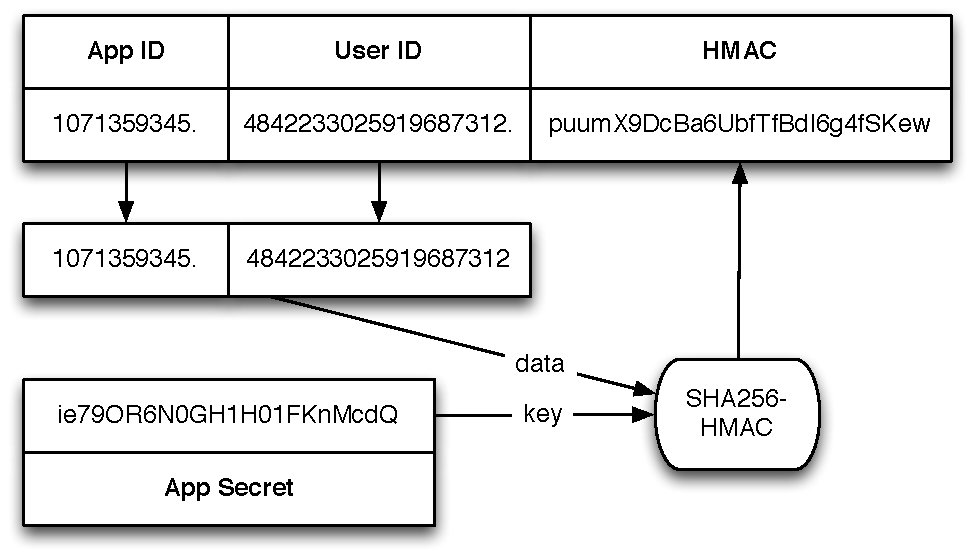
\includegraphics[width=85mm]{figures/user-token.pdf}}
  \caption{
    The algorithm for generating a user token
  }
  \label{fig:user-token}
\end{figure}

The NetMap measurement library embedded in game clients uploads the measurement
data to the NetMap server by sending an HTTP POST request to
\texttt{/readings}. The request body has the JSON data for the measurements,
separated by newlines. The NetMap server parses the JSON on each line,
validates the user tokens in the valid lines, and writes the measurements with
valid tokesn to the database, silently discarding duplicates. The client-side
code runs in a loop that attempts to upload a set of measurements queued in the
database, and removes them from the database if it receives a successful
response (HTTP status code 200 or 400) from the server. We batch multiple
measurements in an HTTP request to amortize the costs of setting up a SSL
connection. Silently discarding duplicates makes the upload request idempotent,
so the process is resilient to network errors. In the presence of client-side
bugs, the NetMap server salvages all the valid measurements.

We have implemented the NetMap server in CoffeeScript, on top of the node.js
platform, using the express.js Web application framework. The server currently
runs on one VM instance in MIT CSAIL's OpenStack cluster.
However, we note that the current
design makes it easy to shard the server in the future, should the need arise.
Each shard would carry a copy of the (relatively small) table of application
IDs and secrets, and would store measurement data received by game clients,
eliminating duplicates. A separate process would centralize the data from all
the shards, and perform a second round of duplicate removal.

\subsection{The Sample Game}

Our source tree includes sample implementations for a game server and client,
in the hope that game developers can use the sample code to accelerate their
development process. Figure \ref{fig:sample} illustrates the components of the
sample game.

\begin{figure}[hbtp]
  \center{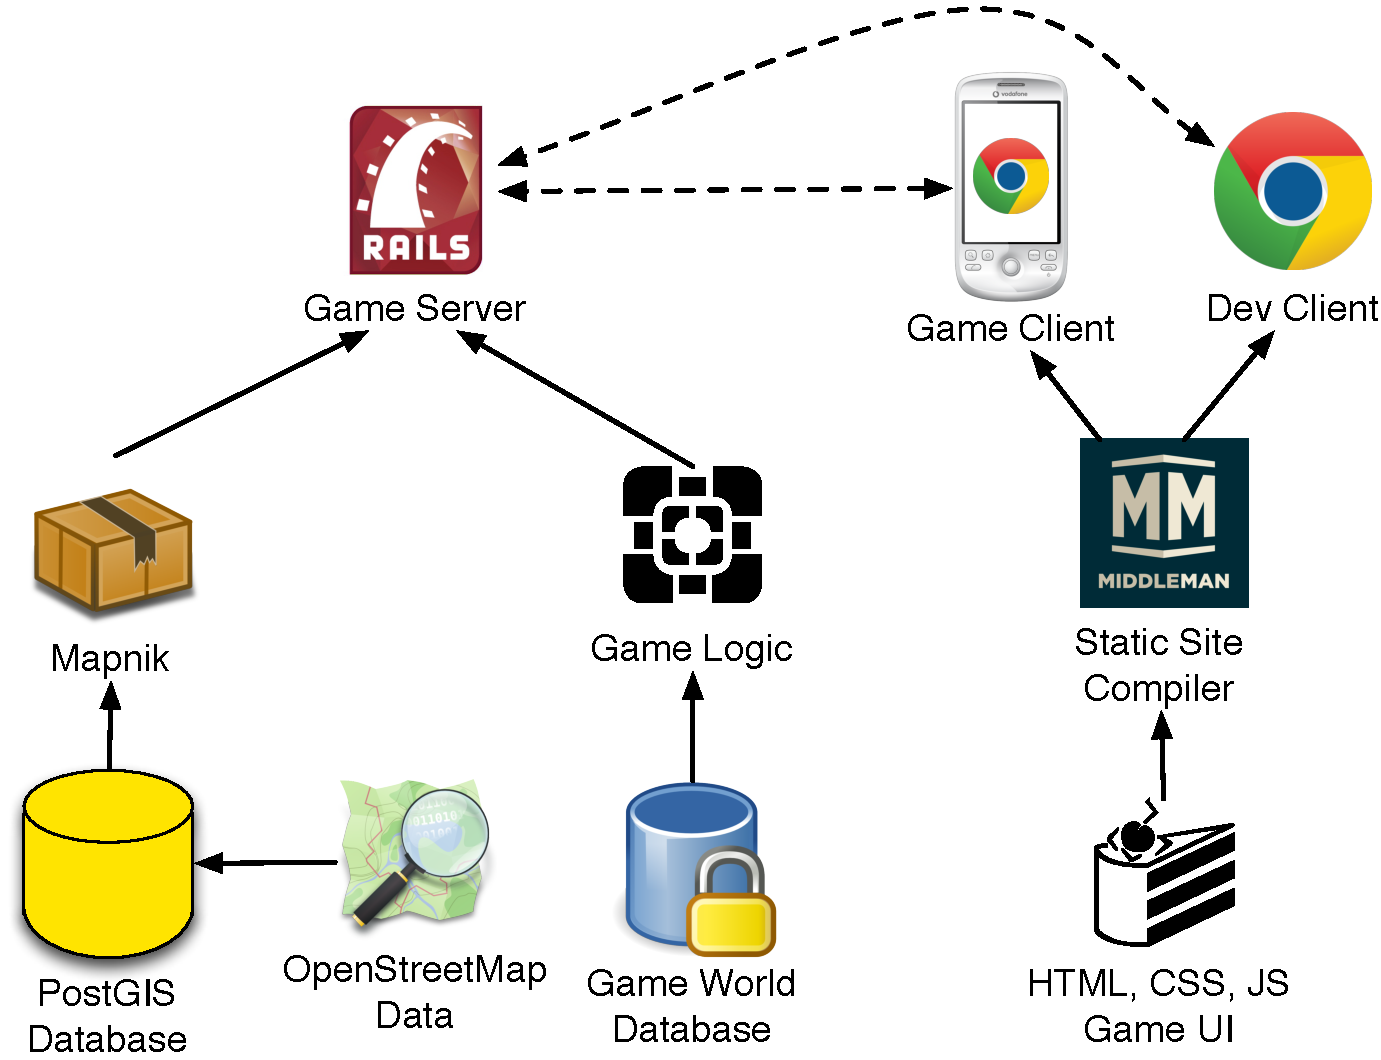
\includegraphics[width=85mm]{figures/gamedev.pdf}}
  \caption{
    The sample game server and client
  }
  \label{fig:sample}
\end{figure}

We imagine that most location-based games will build the in-game map based on
the real-world map, so we provide a pipeline for producing map information that
consists entirely of data and software available under licenses that allow
redistribution. We specifically steered away from mapping platforms with
restrictive licenses, such as Google Maps, in order to avoid having the NetMap
measurement data be considered a derivative of someone else's intellectual
property, which would restrict our ability to make this data available for
research purposes. Our pipeline imports OpenStreetMap data in a PostGIS
database, uses the mapnik library to render map tiles, and uses RubyMapnik
together with Ruby on Rails to serve the map tiles from a HTTP server. The map
tiles in Figures \ref{fig:bw} and \ref{fig:rtt} are rendered using the pipeline
described above.

The sample game server is written in Ruby on Rails, and shows the recommended
method of integrating with the NetMap server. The codebase also includes
straightforward implementations of signup and login pages, player profiles,
a game manual, and integration with the PostGIS for efficient geographical
queries. The game server is packaged together with a development version of the
NetMap server in a VirtualBox VM image, so game developers can start hacking
right away. The VM setup process is fully documented in the form of shell
scripts, which can be used by game developers to set up their own customized
development VMs, and as an inspiration for the production deployment of their
game servers. We used our scripts to set up a production server in a VM
instance on CSAIL's OpenStack infrastructure, and we expect the scripts to work
just as well on Amazon EC2.

The sample game's UI is written completely in HTML, SCSS (a superset of CSS)
and CoffeeScript (a better syntax for JavaScript). We use the Middleman ruby
gem to compile the UI into a static Web site that uses XMLHttpRequest to
interact with the game server. This setup lets game developers iterate on the
game design and logic using Google Chrome and its Developer tools, which yields
a significantly better iteration speed than the standard Android
build-test-deploy process.

The game client contains sample code for connecting to the NetMap measurement
library and ChromeView, our own packaging of the Google Chrome code, with an
API that matches Android's WebKit API. We built ChromeView to ensure a
consistent experience across different Android devices, and so that we don't
have to track bugs that depend on variations in the WebView implementations in
phone firmwares. The API parity with WebView is intentional, as it allows game
developers to remove ChromeView from their games, and still use the rest of our
code with a standard WebView. ChromeView generated some outside interest, and
ended up being a significantly bigger time commitment than initially expected.

The sample game client includes a thin layer of JavaScript bindings that expose
the NetMap measurement library to the JavaScript game logic running inside
ChromeView. The sample game server includes a pure-JavaScript emulation of the
JavaScript bindings that is used when accessing the game from the Google Chrome
browser, during game development. The emulated bindings use standard HTML5
features, such as the XMLHttpRequest, the W3C Geolocation API and IndexedDB, to
implement the NetMap library methods such as \texttt{measure}, \texttt{upload}
and \texttt{location}. Our emulation does not yet collect network performance
measurements, but we are closely watching Google's efforts of implementing the
NDT library in JavaScript.
